

\begin{figure}[h!]
	\centering
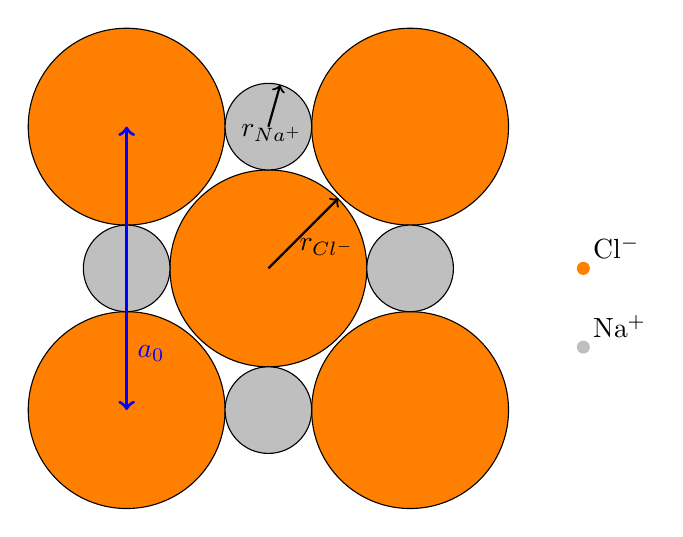
\begin{tikzpicture}
	
	
	
	% Blue Circles
	\foreach \pos in {(0,0) , (-1.8,-1.8), (1.8,1.8), (1.8,-1.8), (-1.8,1.8)} {
		\draw[fill=orange] \pos circle (1.25);
	}
	
	\foreach \pos in {(0,1.8), (0,-1.8), (-1.8,0), (1.8,0) } {
		\draw[fill=gray!50] \pos circle (0.55);
	}
	% Lines
	
	% Légende
	\draw (4, 0) node[circle,fill=orange,scale=0.5] {} node[anchor=south west] {Cl$^-$};  
	
	\draw (4, -1) node[circle,fill=gray!50,scale=0.5] {} node[anchor=south west] {Na$^+$};  
	
	\draw[thick,->, black] (0,0) -- (0.89,0.89) node[pos=0.3,anchor=west]{\(r_{Cl^-}\)};
	
	\draw[thick,->, black] (0,1.8) -- (0.15,2.33) node[pos=0.3,anchor=north]{\(r_{Na^+}\)};
	% Label
	
	\draw[very thick,<->, blue] (-1.8,-1.8) -- (-1.8,1.8) node[pos=0.2,anchor=west]{\(a_0\)};
\end{tikzpicture}
	\caption{\centering Plan (200) du monocristal de NaCl vu de dessus, $r_{Na^+}$ : rayon du cation $Na^+$, $r_{Cl^-}$ : rayon de l'anion $Cl^-$}
	\label{fig:Plan (200) du monocristal de NaCl vu de dessus}
\end{figure}
